\section{Background and Preliminaries}
\label{sec:background}
UPPRESSO is compatible with OIDC and provides privacy protections based on the discrete logarithm problem.
Here, we provide a brief introduction about OIDC and the discrete logarithm problem.

\subsection{OpenID Connect}
\label{subsec:OIDC}
As an extension of OAuth 2.0 to support user authentication, OIDC~\cite{OpenIDConnect} is one of the most popular SSO protocols.
Same as other SSO protocols~\cite{SAMLIdentifier}, OIDC involves three entities, i.e., {\em users}, the {\em identity provider (IdP)}, and {\em relying parties (RPs)}.
Both users and RPs register at the IdP with identifiers ($ID_U$, $ID_{RP}$ and $PID_U$ in some schemes),
  %(or $PID_{RP}$ in some schemes)
   and the necessary information such as credentials, RP endpoints (e.g., URLs to receive the identity proofs), etc.
% below can be removed
The IdP is assumed to maintain these attributes securely.
In an OIDC login process, a user is responsible for initiating a login request at an RP, redirecting the SSO messages between the RP and IdP, and checking the scope of user attributes in the identify proof generated by the IdP for the visited RP.
Usually, the redirection and checking actions are handled by a user-controlled software,
 known as {\em user agent} (e.g., browser).
Once receiving a user login request, the RP constructs an identity proof request with its identifier and the requested scope of user attributes,
 sends the identity proof request to the IdP through the user, and parses the received identity proof to authenticate the user.
The IdP authenticates the user based on her $ID_U$ and credential,
 maps $ID_U$ to $PPID$ (i.e., privacy-preserving pseudo-identifier) based on the RP identity ($ID_{RP}$),
 generates an identity proof containing $PPID$, $ID_{RP}$ and requested user attributes,
  and returns the identity proof to the endpoint registered by the RP.

\vspace{1mm}\noindent\textbf{OIDC Implicit Flow.}
 OIDC supports three different user login flows, which are the {\em implicit flow}, {\em authorization code flow} and {\em hybrid flow} (i.e., a mix-up of the previous two).
 In the implicit flow, an {\em id token} is generated as the identity proof, which contains a user identifier, an RP identifier,
    the issuer (i.e., IdP), the validity period, and other requested attributes.
The IdP signs the id token using its private key to ensure integrity, and sends it to RP through the user.
In the authorization code flow, the IdP binds an authorization code with the RP, and sends it to the RP through the user;
then, the RP establishes an HTTPS connection to the IdP %to ensure the integrity and confidentiality of the identity proof,
    and uses the authorization code with the RP's credential to obtain the user's identifier and other attributes.
UPPRESSO is compatible with all three flows. For brevity, we will present our design and implementation of UPPRESSO on top of the implicit flow of OIDC in details, and discuss the extension to support the authorization code flow in Section~\ref{sec:discussion}.

The original OIDC implicit flow is shown in Figure~\ref{fig:OpenID}. When a user attempts to log into an RP,
    the RP constructs an identity proof request and returns it to the user, which gets redirected to the IdP.
The request contains $ID_{RP}$, the RP endpoint to receive the identity proof, and the scope of requested user attributes.
If the user has not yet been authenticated, the IdP initiates an authentication process to authenticate her.
For a successfully authenticated user, the IdP generates an id token  and returns it to the RP endpoint.
If the endpoint is not registered for that RP,
    the IdP will return a warning to notify the user about potential identity proof leakage.
Once the RP receives the identity proof, it makes the authentication decision after verifying the validity.
%extracts user's identifier and returns the authentication result to the user (Step 7).

\vspace{1mm}\noindent\textbf{RP Dynamic Registration.} The RP dynamic registration~\cite{DynamicRegistration} of OIDC allows an RP to update its information at the IdP. When an RP first registers at the IdP, it obtains a registration token, with which the RP can initiate a dynamic registration process to update its information (e.g., the endpoint).
After a successful dynamic registration, the RP obtains a new unique $ID_{RP}$ from the IdP.
UPPRESSO leverages this function and slightly modify the dynamic registration process to enable {\em RP pseudo-identifier registration},
 which allows an RP to generate different privacy-preserving identifiers ($PID_{RP}$s) and register them at the IdP.

\begin{figure}[t]
  \centering
  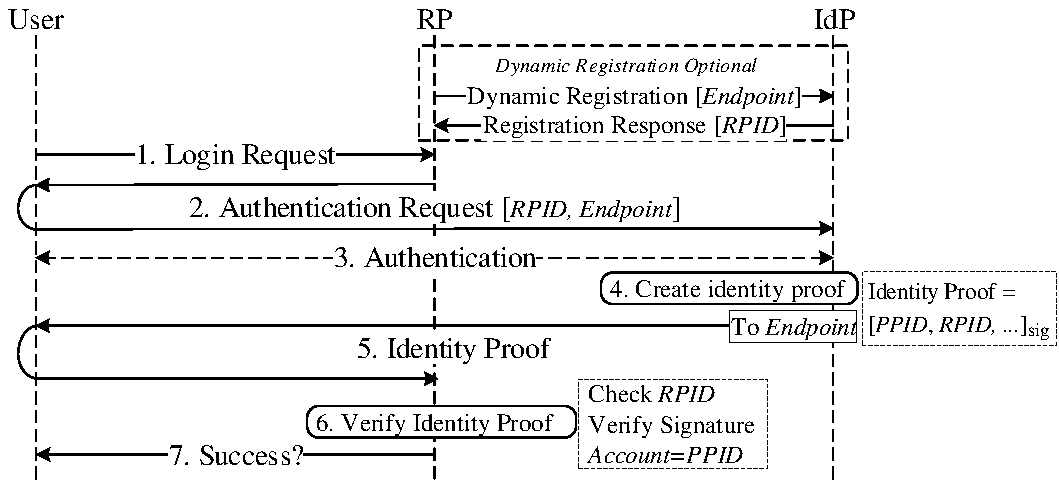
\includegraphics[width=0.95\linewidth]{fig/OIDC1.pdf}
  \caption{The implicit flow of OIDC.}
  \label{fig:OpenID}
\end{figure}

\subsection{Discrete Logarithm Problem}
\label{sec:dlp}

Based on the discrete logarithm problem, UPPRESSO design the identifier-transformation functions. %$\mathcal{F}_{ID_{RP} \mapsto PID_{RP}}$ and $\mathcal{F}_{ID_{U} \mapsto PID_{U}}$ to generate privacy-preserving user identifier (e.g. $PID_U$) and RP identifier (e.g. $PID_{RP}$), respectively.
Here, we briefly review the discrete logarithm problem.

%A number $g$ ($0<g<p$) is called a primitive root modular a prime $p$, if for ${\forall}y$ ($0<y<p$), there is a  number $x$ ($0\le x <p-1$) satisfying $y=g^x \pmod p$.
For the finite field $GF(p)$ where $p$ is a large prime, a number $g$ is called a generator of order $q$, if it constructs a cyclic  group of $q$ elements by calculating $y=g^x \ mod\ p$.
And, $x$ is called the discrete logarithm of $y$ modulo $p$. Given a large prime $p$, a generator $g$ and a number $y$, it is computationally infeasible to solve the discrete logarithm (i.e., $x$) of $y$~\cite{WXWM}, which is called the discrete logarithm problem.
The hardness of solving discrete logarithms is utilized to design several secure cryptographic primitives, including Diffie-Hellman key exchange and the digital signature algorithm (DSA).

%In the process of $F_{PID_{RP}}$ and $F_{PID_U}$, we needs to calculate the primitive root for a  large prime $p$ as follows~\cite{Shoup,Wang}. First, we retrieve a primitive root $g_m$  modulo $p$ from all the integers by finding the first integer passing  the primitive root checking.  A lemma is propose to simply the checking, that if $p=2q+1$ ($q$ is a prime),  an integer $\mu \in (1, p-1)$ is a primitive root if and only if $\mu^2\neq 1 \ mod \ p$ and $\mu^q\neq 1 \ mod \ p$. Then, based on $g_m$, we can calculate a new primitive root $g = g_{m}^{t} mod \ p$, where $t$ is an integer coprime to $p-1$.
